\chapter{Introduction}

Perhaps only in passing, many of us have seen images of the periodic table (Figure \ref{fig:periodictable}) 

 good place to start is with H$_{2}$O, colloquially called water. It consists of two hydrogen atoms and one oxygen atom.

The objects responsible for chemistry are found in the periodic table of the elements seen in Figure \ref{fig:periodictable}. Quantum mechanics was developed in the early 20th century and gave an explanation for the experimentally determined structure to the period table of elements.

\begin{figure}[htbp]
\centering
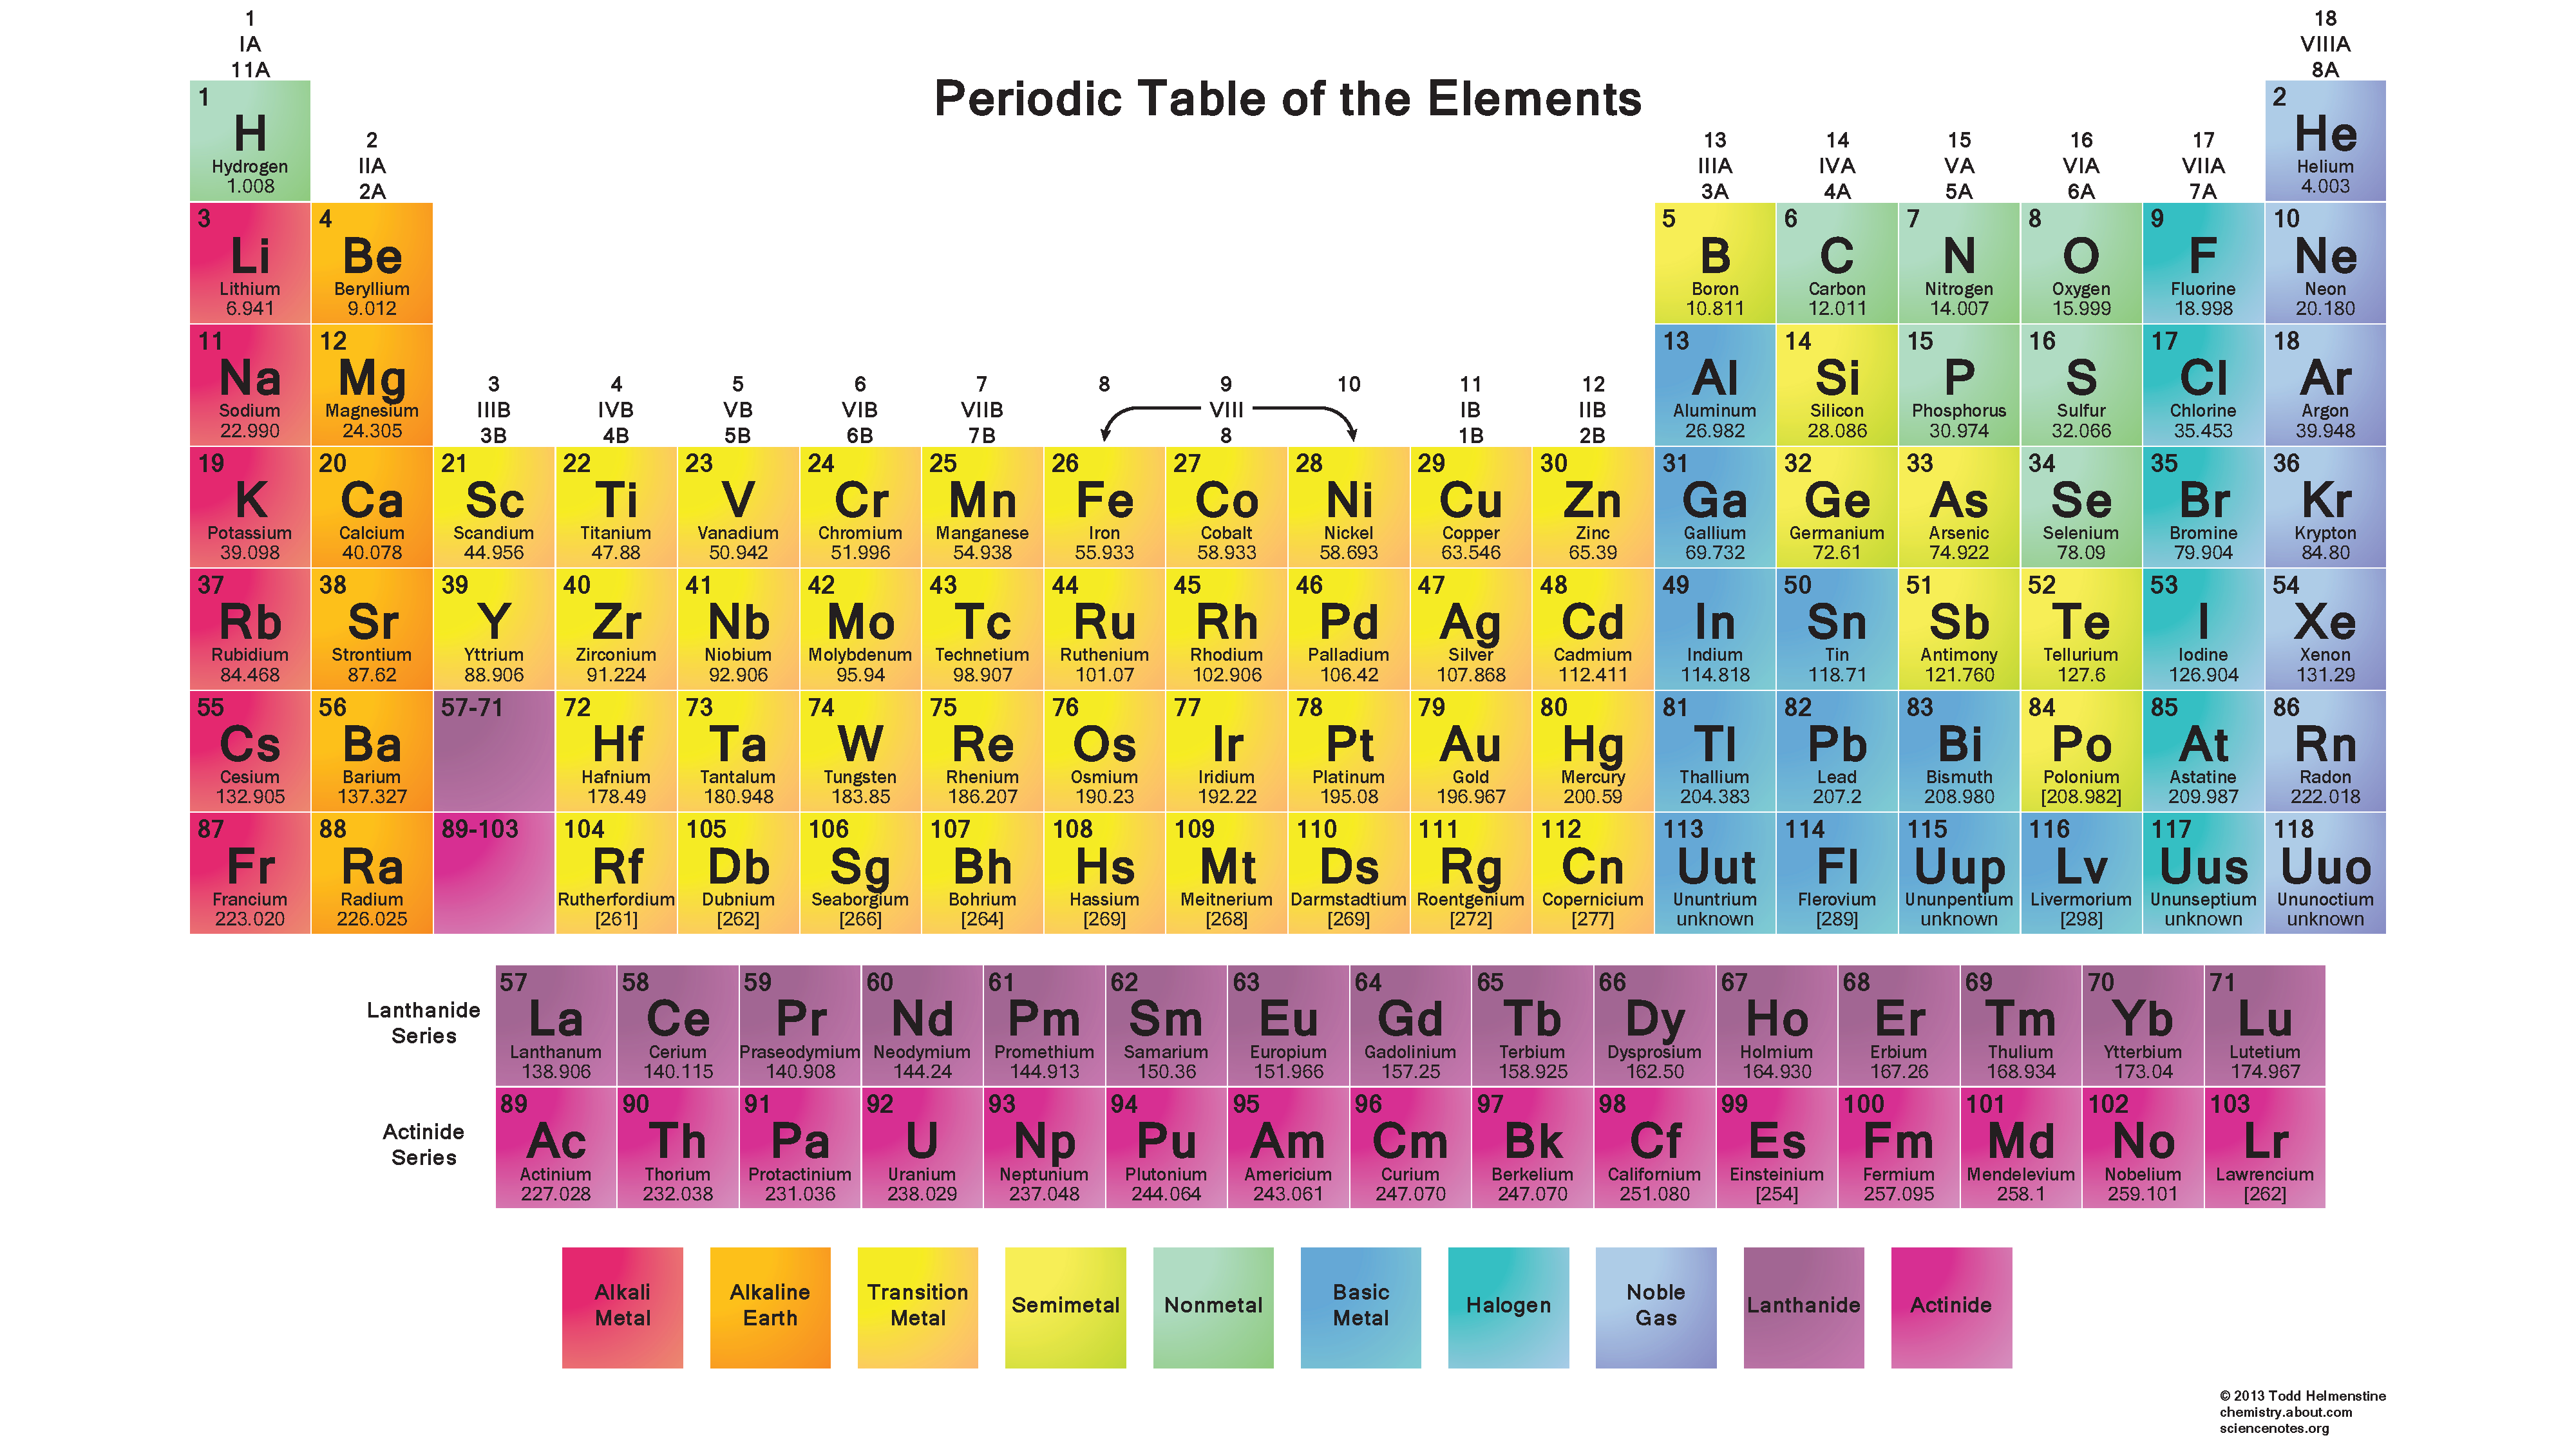
\includegraphics[width=0.8\textwidth]{figs/PeriodicTable.pdf}
\caption{The periodic table of elements.}
\label{fig:periodictable}
\end{figure}

But the elements themselves are made of more fundamental ``atoms'' described by the Standard Model of particle physics, the current knowledge is summarized in another table, seen in Figure \ref{fig:sm}.

This thesis gives an overview  presents current research in the field of particle physics. A description of the Standard Model is presented in Chapter \ref{chap:sm}. A description of the Large Hadron Collider (LHC) is presented in Chapter \ref{chap:lhc}. A description of the CMS detector is presented in Chapter \ref{chap:detector}. A description of the object definition and event reconstruction is presented in Chapter \ref{chap:eventreco}.  A description of the physics analysis is presented in Chapter \ref{chap:analysis}. The conclusions are discussed in Chapter \ref{chap:conclusions}.
